\section{Updated Migovec Exploration Summary}

The original \passage{Migovec} discoveries were by the JSPDT in the 1970s (\passage{M2},
-350m) and 1980s (\passage{M16}, -547m). ICCC has been going on regular expeditions
to \passage{Migovec} since 1994. With the JSPDT this including the finding of
\passage{M18} which was connected into \passage{M2} and \passage{M16} in 1996. This system (\passage{SysMig})
was explored to chokes at -937 m and -958 m and sumps at -970 m and -967 m (the sumps are at 885 m above sea level). \passage{SysMig} is 11.5 km
in length; most of this length is due to the many vertical shafts (\bignote{vertical length of survey is 6.8 km}).

The focus of expeditions shifted to \passage{Vrtnarija} in 2000, which was discovered
and pushed down to -802m by 2004. This cave was initially thought to be much more linear than \passage{SysMig}, having a typical vertical entrance
series to -550 m, where a large horizontal phreatic (\passage{Friendship Gallery}) led to a pitch (\passage{Big Rock Candy Mountain}) down to an extensive horizontal level. No true sumps were discovered; the cave was pushed to reach a mud sump with tiny flow.

\begin{center}
\begin{pagefigure}
\centering
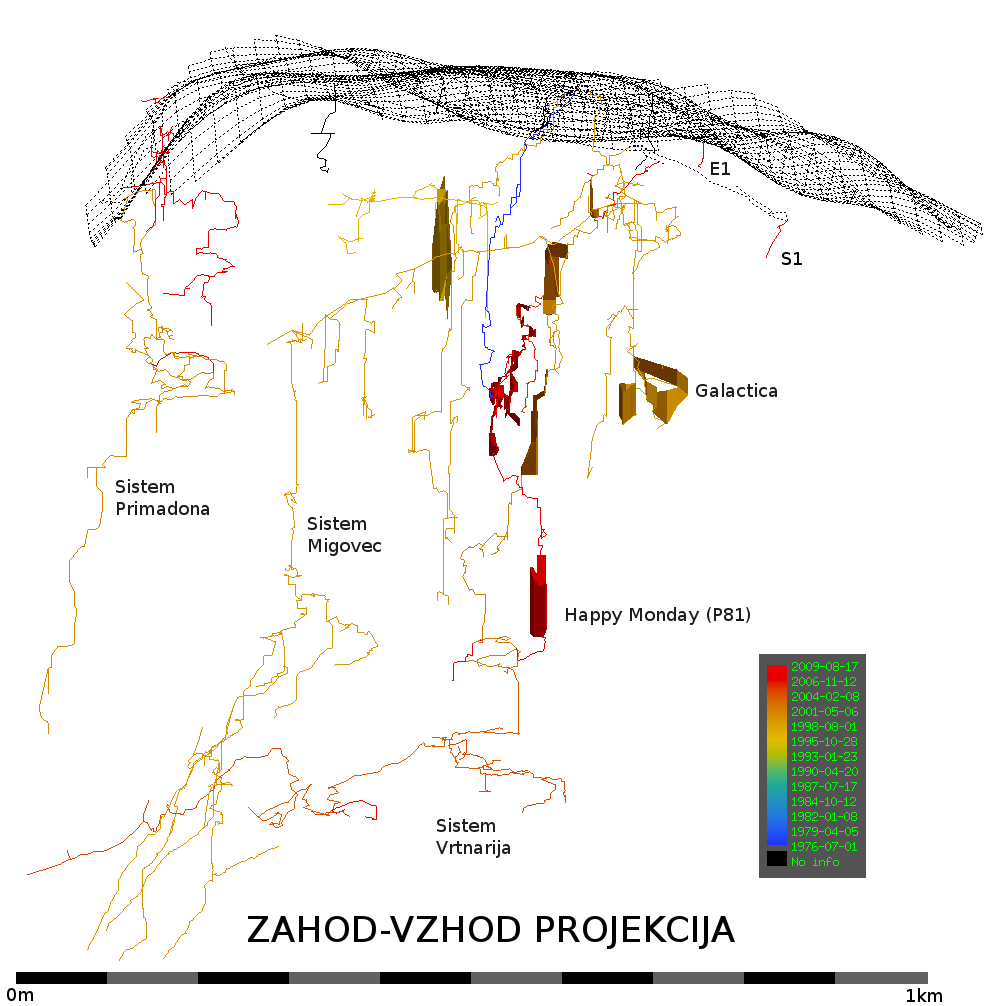
\includegraphics[width=0.75\columnwidth]{2010/mig_background2010/mig_2009_for_jamar.png}
\caption{A West---East projection of the 2009 extent of known cave passage within \passage{Migovec}, with surface topology
(Digital Elevation Model from Slovene Karst Institute).}
\end{pagefigure}
\end{center}

\newpage


During the 2005 and 2007 expeditions a small side passage in \passage{Vrtnarija}
(\passage{Captain Kangaroo}) was pushed. Analysis of the survey data before
summer 2008 suggested that this passage was within 50 m of the \passage{M2}
part of \passage{SysMig}, which no one had been down since the 1970s. Connection
of \passage{SysMig} to \passage{Vrtnarija} would form the largest alpine system in Slovenia.

During the 2008 expedition, \passage{M2} was rerigged. Exploration in \passage{Vrtnarija}
was concentrated within the 'depth range' of a possible \passage{M2} connection
(the best vertical lead, \passage{Dark Tranquillity}, was abandoned at -338 m).
\passage{M2}, which closes down enormously after -250 m, was slowly pushed with
extension persuasion. 

In 2009, a camp was made in \passage{Vrtnarija} near the potential connection
to \passage{M2}. Several climbs and other 'secondary' leads in the vicinity
of camp were probed, without finding the connection. \passage{Dark Tranquillity}
was pushed well below the bottom of \passage{M2}. This connected to a passage underneath
\passage{Friendship Gallery} (\passage{Falls Road}, a small confluence). 
On a trip to rig ropes from \passage{Friendship Gallery} to allow the physical
connection, an old lead (\passage{Korita}) was looked at and proved viable.

At the beginning of the 2010 expedition, the known length of \passage{Vrtnarija} was 6.575 km.

\begin{pagefigure}
\checkoddpage \ifoddpage \forcerectofloat \else \forceversofloat \fi
\centering
 \frame{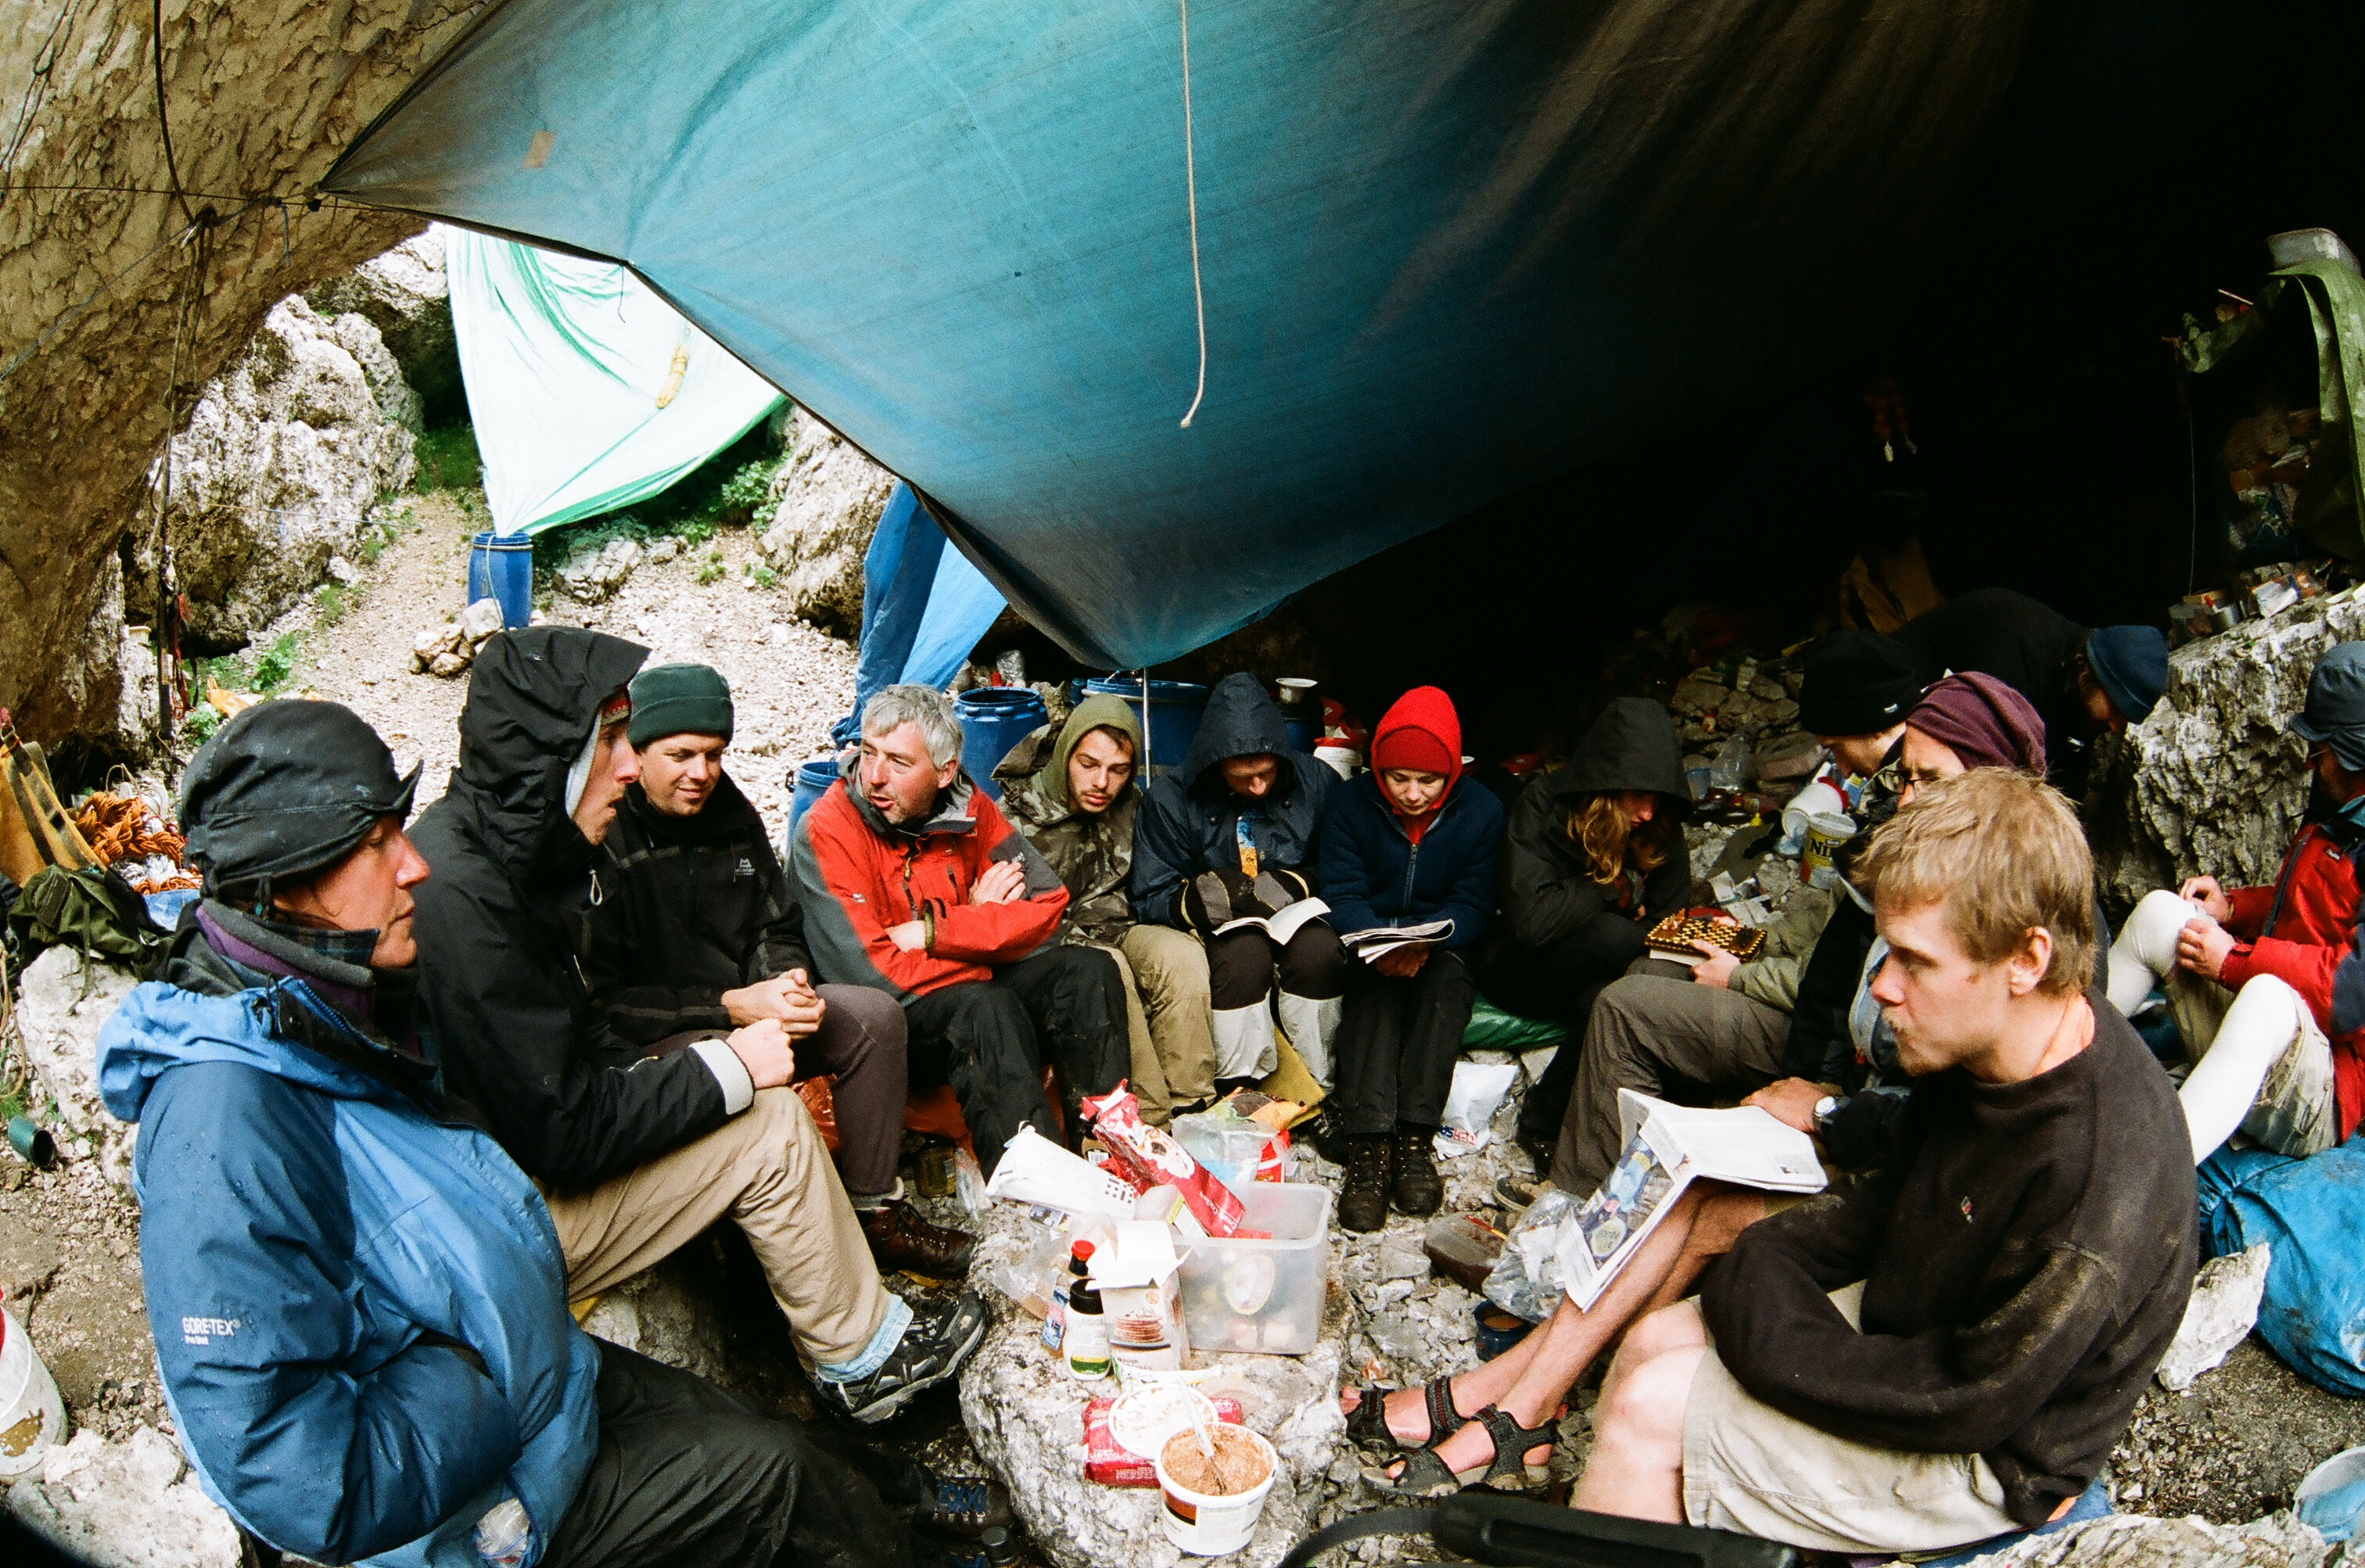
\includegraphics[width=\textwidth]{2010/mig_background2010/Jarvist Frost - Canon A1 Zenit 16mm - 61320031--orig.jpg}} 
 \caption{Wet days - of which there were many in 2010 - lead to mass sheltering in the bivi to keep warm and dry (relatively speaking). \pic{Jarvist Frost}}
 \label{wet bivi 2010}
\end{pagefigure}
